\subsection{Embedding contestualizzati: BERT}
I modelli statici come GloVe presentano diverse limitazioni:
\begin{itemize}
    \item L'uso di modelli linguistici molto superficiali. Questo significa che c'è un limite alla quantità di informazioni che possono catturare.
    \item Un'altra limitazione chiave è che questi modelli non prendono in considerazione il contesto della parola: questi modelli producono un solo embedding per ogni parola, combinando tutti i diversi sensi della parola in un unico vettore.
\end{itemize}
Alla fine del 2018 i ricercatori di Google AI Language hanno reso open-source una nuova tecnica per l'elaborazione del linguaggio naturale (NLP) chiamata \textbf{BERT (Bidirectional Encoder Representations from Transformers)} - una grande svolta che ha preso d'assalto la comunità del Deep Learning per le sue incredibili prestazioni. Il team di ricerca che ha lavorato dietro BERT lo descrive così:
\begin{center}
    \textit{"BERT sta per Bidirectional Encoder Representations from Transformers.  È progettato per pre-addestrare rappresentazioni bidirezionali profonde da testi non etichettati, condizionando congiuntamente il contesto sinistro e destro. Come risultato, il modello BERT pre-addestrato può essere messo a punto con un solo strato di output aggiuntivo per creare modelli all'avanguardia per una vasta gamma di compiti NLP."}
\end{center}
In primo luogo, BERT è basato sull'architettura \textbf{Transformer}, un modello proposto nel paper \textit{Attention is All You Need}\textsuperscript{\cite{vaswani2017attention}} che usa l'\textit{attenzione} (successore del modello sequence-to-sequence) per accelerare il processo di addestramento. In secondo luogo, BERT è pre-addestrato su un grande corpus di testo non etichettato che include l'intera \textbf{Wikipedia} (2.500 milioni di parole) e il Book Corpus (800 milioni di parole). In terzo luogo, BERT è un modello \textit{"profondamente bidirezionale"}. Bidirezionale significa che BERT apprende informazioni sia dal lato sinistro che da quello destro del contesto di un token durante la fase di formazione.

Il paper pubblicato dai creatori di Bert, presenta due modelli che si differenziano per le loro dimensioni: \begin{itemize}
    \item \textbf{BERT Base}: 12 strati (blocchi di trasformatori), 12 teste di attenzione e 110 milioni di parametri
    \item \textbf{BERT Large}: 24 strati (blocchi di trasformatori), 16 teste di attenzione e 340 milioni di parametri
\end{itemize}
\begin{figure}[hbt!]
    \centering
    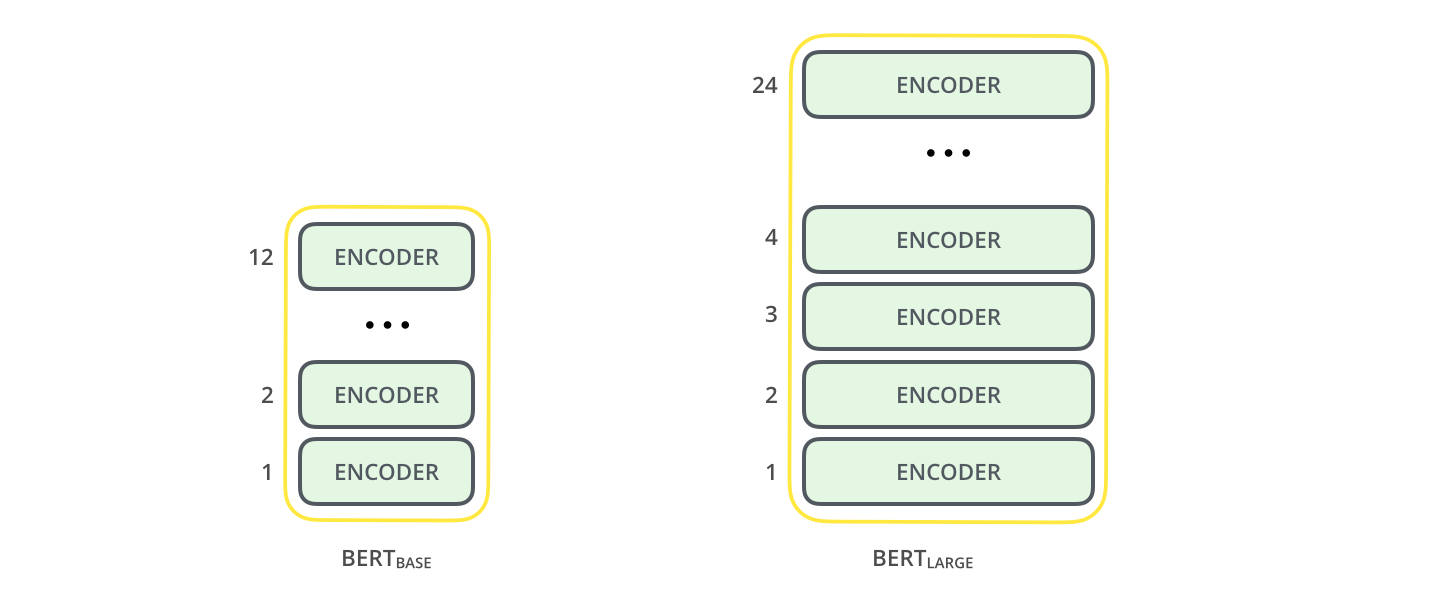
\includegraphics[width=1\textwidth]{img/bert_architecture.png}
    \caption{BERT Base e BERT Large}
    \label{fig:bert_architettura}
\end{figure}
\newpage
BERT è pre-addestrato su due compiti NLP:
\begin{itemize}
    \item \textbf{Masked Language Model}: Viene utilizzato per addestrare la capacità di BERT di catturare informazioni in maniera bidirezionale. Data una frase, il 15\% di essa viene \textit{mascherato} usando token speciali (ad esempio "[MASK]") e viene chiesto di prevedere la parola corretta che dovrebbe trovarsi in quella posizione. Durante l'addestramento di BERT viene utilizzata la seguente tecnica:
    \begin{enumerate}
        \item L'80\% delle volte le parole sono state sostituite con il token mascherato [MASK].
        \item Il 10\% delle volte le parole sono state sostituite con parole casuali.
        \item Il 10\% delle volte le parole sono rimaste invariate.
    \end{enumerate}
    \item \textbf{Next Sentence Prediction}: Questo è un task di classificazione binaria che viene utilizzato per addestrare BERT, in modo tale che quest'ultimo possa essere utilizzato in compiti nei quali è necessario sapere comprendere le relazioni che intercorrono tra le frasi. Il quesito posto è: date due frasi A e B prese da un corpus linguistico, determinare se la frase B segue la frase A nel testo oppure no.   
    \begin{enumerate}
        \item Per il 50\% delle coppie, la seconda frase sarebbe in realtà la frase successiva alla prima.
        \item Per il restante 50\% delle coppie, la seconda frase sarebbe una frase casuale dal corpus.
    \end{enumerate}
\end{itemize}